% Multi-Model AI Deliberation for Complex Engineering Decisions
% Target: IEEE Intelligent Systems
% Version L — March 2026
% Compile with: pdflatex -> bibtex -> pdflatex -> pdflatex

\documentclass[11pt,a4paper]{article}

% --- Packages ---
\usepackage[margin=2.5cm]{geometry}
\usepackage{amsmath,amssymb}
\usepackage{booktabs}
\usepackage{graphicx}
\usepackage{listings}
\usepackage{xcolor}
\usepackage{hyperref}
\usepackage{authblk}
\usepackage{setspace}
\usepackage{enumitem}
\usepackage{float}
\usepackage{caption}
\usepackage{subcaption}
\usepackage{textcomp}

\graphicspath{{figures/}}

% --- Hyperref configuration ---
\hypersetup{
    colorlinks=true,
    linkcolor=blue!60!black,
    citecolor=blue!60!black,
    urlcolor=blue!60!black,
}

% --- Listings configuration for YAML ---
\lstdefinelanguage{yaml}{
  keywords={true,false,null,y,n},
  keywordstyle=\color{darkgray}\bfseries,
  basicstyle=\ttfamily\small,
  sensitive=false,
  comment=[l]{\#},
  morecomment=[s]{/*}{*/},
  commentstyle=\color{gray}\ttfamily,
  stringstyle=\color{blue!60!black}\ttfamily,
  moredelim=[l][\color{orange}]{:},
  moredelim=[l][\color{teal}]{-\ },
  frame=single,
  framesep=3pt,
  breaklines=true,
  showstringspaces=false,
  columns=fullflexible,
}

\lstset{
  basicstyle=\ttfamily\small,
  frame=single,
  breaklines=true,
  showstringspaces=false,
  columns=fullflexible,
}

% --- Title and Authors ---
\title{\textbf{Multi-Model AI Deliberation for Complex Engineering Decisions: A Structured Methodology with Divergent View Preservation}}

\author{Project Dyson Research Team\thanks{This paper was produced with AI assistance. The deliberation system uses commercially available large language models (Claude 4.6, Gemini 3 Pro, GPT-5.2) accessed through Databricks serving endpoints. Full AI involvement disclosure is provided in the Ethics Statement (Section~\ref{sec:ethics}).}}

\affil{Project Dyson --- Open-Source Space Infrastructure Initiative\\ \texttt{https://projectdyson.org}}

\date{March 2026}

\begin{document}

\maketitle

% ============================================================
% ABSTRACT
% ============================================================
\begin{abstract}
We present a structured methodology for multi-model engineering deliberation in which multiple large language models independently generate proposals, evaluate each other's work through weighted voting, and iterate toward conclusions while preserving disagreements as machine-readable artifacts. The methodology's most distinctive contribution is its treatment of disagreement as information: a divergent views schema captures model attribution, evidence, and resolution status for each persisting disagreement. We illustrate the methodology through 16~architectural trade studies for a space infrastructure project, with repeated trials ($n = 5$ independent runs on 4~stratified questions at $T = 0.7$) establishing reliability: round-winner identity is stable across 85\% of trials (range: 60--100\%), convergence rounds vary within $\pm 1$ of the median, and termination conditions are reached unanimously in 95\% of runs. Transcript-based similarity analysis across six semantic metrics characterizes deliberation dynamics: all metrics \emph{decrease} across rounds, with the largest decreases in decision-sentence TF-IDF ($\Delta = -0.031$) and technical parameter Jaccard ($\Delta = -0.064$), consistent with genuine refinement though not definitive. Commitment-level tracking confirms that the Round~1 winner maintains its own commitments more strongly (mean cosine = 0.208) than non-winners adopt them (mean = 0.164), consistent with genuine refinement rather than sycophancy. Controlled experiments comparing deliberation against aggregation-only and single-model self-refinement baselines across 15--16 questions show comparable quantitative output structure, with the distinctive contribution of deliberation being the cross-model divergent views artifact and peer evaluation process. A divergent view extraction experiment on aggregation-only proposals reveals that aggregation captures 10.8~topics per question (78\% genuine trade-offs) versus deliberation's 2.9 (26\% genuine trade-offs), reflecting the distinction between enumerating all initial disagreements and curating only those that persist after iterative convergence. Across 16~deliberations, 47~divergent topics were identified, of which 12 were confirmed as genuine engineering trade-offs through literature review.

\medskip
\noindent\textbf{Keywords:} multi-agent systems, large language models, engineering design, structured deliberation, divergent views, design rationale, Delphi method
\end{abstract}

\onehalfspacing

% ============================================================
% 1. INTRODUCTION
% ============================================================
\section{Introduction}
\label{sec:introduction}

Complex engineering decisions---selecting between competing architectures, sizing parameters under deep uncertainty, resolving cross-disciplinary trade-offs---traditionally require expert panels. Whether conducted through formal trade studies, design review boards, or structured consensus methods such as the Delphi technique~\cite{linstone1975delphi}, these processes are expensive, slow, and subject to well-documented social dynamics including groupthink~\cite{janis1982groupthink} and anchoring effects. In preliminary design phases, where dozens of architectural questions must be explored before any can be definitively answered, the cost of assembling expert panels for each question is often prohibitive.

Frontier large language models (LLMs)---here denoting the most capable commercially available models from distinct model families at the time of the study---have demonstrated substantial competence in technical reasoning across engineering domains~\cite{bubeck2023sparks,openai2024gpt4}. While no individual model matches a domain expert's depth of specialized knowledge, different model families exhibit measurably different reasoning styles, knowledge emphases, and failure modes. These differences---often treated as a nuisance in benchmarking contexts---represent a potential resource: systematic diversity in engineering judgment that can be harnessed through structured deliberation.

Yet existing work on multi-agent LLM systems focuses predominantly on conversational games~\cite{du2023debate}, natural language tasks~\cite{wu2023autogen}, or evaluation frameworks~\cite{zheng2024judging}. To our knowledge, no structured methodology has been published for multi-model deliberation on engineering trade studies---problems where multiple valid approaches exist and the preservation of minority positions is as valuable as convergence.

This paper makes three specific contributions: (1)~the first application of structured multi-model LLM deliberation to engineering trade studies, adapting the computational Delphi paradigm to heterogeneous AI models; (2)~the divergent views schema, a structured representation for preserving attributed disagreements with evidence and resolution status as a first-class design rationale artifact; and (3)~empirical characterization of multi-model deliberation dynamics, including convergence behavior, voting patterns, and transcript-based similarity analysis across 16 engineering questions.\footnote{Individual author names and affiliations will be provided for final publication.}

% ============================================================
% 2. RELATED WORK
% ============================================================
\section{Related Work}
\label{sec:related}

\textbf{Multi-agent LLM systems.} The ``wisdom of crowds'' literature~\cite{surowiecki2004wisdom} identifies conditions---diversity, independence, decentralization---under which group aggregation outperforms individual judgment. Irving et al.~\cite{irving2018debate} proposed AI safety via debate, demonstrating that adversarial dynamics improve truthfulness. Du et al.~\cite{du2023debate} showed that multi-agent debate improves factual accuracy through counterarguments. Wu et al.~\cite{wu2023autogen} developed AutoGen for multi-agent conversation, while Zheng et al.~\cite{zheng2024judging} established LLM-as-judge evaluation. Liang et al.~\cite{liang2024encouraging} explored multi-agent debate for divergent thinking, and Chan et al.~\cite{chan2024chateval} proposed ChatEval for multi-agent evaluation. Wang et al.~\cite{wang2024rethinking} examined the bounds of LLM reasoning through multi-agent discussions, finding that benefits depend heavily on task characteristics and discussion structure. A complementary line of work explores single-model self-refinement: Madaan et al.~\cite{madaan2023self} demonstrated that LLMs can iteratively improve outputs through self-generated feedback without multi-model interaction. Perez et al.~\cite{perez2022sycophancy} developed model-written evaluations that systematically probe LLM behaviors including sycophancy, while Sharma et al.~\cite{sharma2024sycophancy} provided a systematic study showing that models tend to align with user preferences even when doing so is incorrect---concerns directly relevant to multi-model deliberation where models see each other's outputs. These contributions target natural language tasks rather than engineering trade studies, where no single correct answer exists and multiple valid approaches must be compared along incommensurable dimensions~\cite{keeney1976decisions}.

\textbf{Expert consensus methods.} The Delphi method~\cite{linstone1975delphi,dalkey1963experimental}---anonymous proposals, structured feedback between rounds, iterative convergence, and statistical aggregation---bears striking parallels to our methodology. Nominal Group Technique~\cite{delbecq1975group} adds structured turn-taking, while the RAND/UCLA Appropriateness Method~\cite{fitch2001rand} applies Delphi-like processes to medical decision-making. These methods typically require 3--4 rounds for convergence, involve 7--15 panelists, and take weeks to months. Our system can be understood as a computational analogue, with LLMs replacing human experts, structured voting replacing questionnaires, and machine-readable divergent views replacing statistical dispersion measures. The key innovation is that our system preserves and categorizes disagreements as first-class outputs rather than treating them as noise.

\textbf{Engineering trade study methods.} Pugh's concept selection~\cite{pugh1991total}, the Analytic Hierarchy Process~\cite{saaty1980ahp}, and Multi-Attribute Utility Theory~\cite{keeney1976decisions} formalize multi-criteria evaluation. Our methodology differs in generating alternatives and criteria simultaneously through LLM proposals. The divergent views schema extends the design rationale tradition (DRL~\cite{lee1991drl}; QOC~\cite{maclean1991qoc}) by automating capture through multi-model deliberation with model attribution.

\textbf{Structured disagreement.} Red teaming~\cite{zenko2015red}, devil's advocacy~\cite{schwenk1990effects}, and scenario planning~\cite{schwartz1996art} recognize that premature consensus suppresses information. In the machine learning literature, Lakshminarayanan et al.~\cite{lakshminarayanan2017simple} demonstrated that disagreement among ensemble members provides a well-calibrated measure of epistemic uncertainty---a principle we extend from predictive models to deliberative agents. The epistemology of disagreement~\cite{christensen2013epistemology} provides theoretical grounding: when epistemic peers disagree, the disagreement itself constitutes evidence that should be preserved rather than resolved through averaging. Our innovation is making disagreement machine-readable with explicit model attribution, evidence, and resolution status.

% ============================================================
% 3. METHODOLOGY
% ============================================================
\section{Methodology}
\label{sec:methodology}

\subsection{System Architecture}
\label{sec:architecture}

The deliberation system comprises three layers (Fig.~\ref{fig:architecture}). The \emph{model layer} consists of three frontier LLMs accessed through a unified API gateway (Databricks serving endpoints): Claude~4.6 (Anthropic), Gemini~3~Pro (Google DeepMind), and GPT-5.2 (OpenAI).\footnote{Endpoint names: \texttt{databricks-claude-opus-4-6}, \texttt{databricks-gemini-3-pro}, \texttt{databricks-gpt-5-2}. We acknowledge that model versioning in the rapidly evolving LLM ecosystem can be ambiguous; model weights served may differ from providers' direct APIs. All transcripts are archived for post-hoc verification.} The choice of three models balances diversity against coordination complexity; with fewer than three, meaningful voting dynamics cannot emerge, while more than three increases orchestration overhead with diminishing marginal diversity.

The \emph{orchestration layer}, implemented as a Node.js application (\texttt{run-discussion.js}, $\sim$940 lines), manages prompt construction, parallel response collection, structured vote tabulation, and termination condition evaluation. All models operate at temperature $T = 0.7$ to balance creativity with coherence.

The \emph{output layer} produces four artifact types: per-model proposals (markdown), voting records (YAML with per-vote justifications), synthesized conclusions, and divergent views (YAML with model attribution and resolution status). All artifacts are version-controlled alongside the engineering specifications they inform.

\begin{figure}[t]
    \centering
    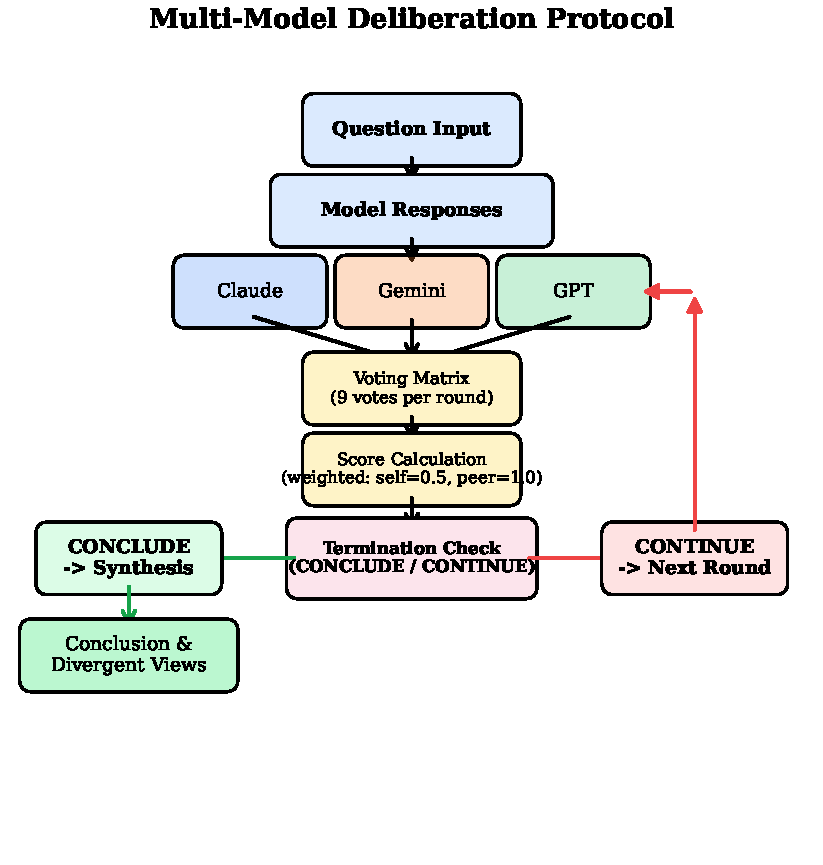
\includegraphics[width=\textwidth]{fig-system-architecture.pdf}
    \caption{Three-tier deliberation architecture. The model layer dispatches prompts to three LLMs through a unified API gateway. The orchestration layer manages prompts, responses, votes, and termination. The output layer produces proposals, voting records, conclusions, and machine-readable divergent views.}
    \label{fig:architecture}
\end{figure}

\subsection{Round Structure}
\label{sec:rounds}

Each round consists of three phases executed sequentially.

\textbf{Proposal generation.} Each model receives: (a)~the research question title and full background context, (b)~prior-round proposals and voting results if applicable (truncated to 1{,}000 words via head truncation, retaining framing and primary specifications), and (c)~guidelines specifying a 2{,}000-word maximum. Models generate free-form technical proposals without structural constraints beyond the word limit, enabling each model to emphasize aspects it considers most important. The prompt for rounds after the first includes the identity and score of the prior round's winning proposal, creating an informed iteration dynamic. We did not test alternative truncation strategies (e.g., model-based summarization), which represents an uncontrolled variable.

\textbf{Peer evaluation.} Each model evaluates all three proposals (including its own) using a three-level scale: APPROVE (2~points), NEUTRAL (1~point), REJECT (0~points). Self-voting is permitted but weighted at $0.5\times$ to preserve the self-assessment signal while preventing self-promotion from dominating. Each vote must be accompanied by a written justification in structured JSON. The weighted score is:
\begin{equation}
    S_i = \sum_{j \neq i} v_{ji} + 0.5 \cdot v_{ii}
    \label{eq:score}
\end{equation}
where $v_{ji} \in \{0, 1, 2\}$ is the score assigned by model $j$ to proposal $i$ (0 = REJECT, 1 = NEUTRAL, 2 = APPROVE). Ties are broken by APPROVE count; persistent ties favor the prior-round winner.

\textbf{Iteration decision.} Each model casts a binary CONTINUE/CONCLUDE vote. Termination occurs when: (1)~all three models vote CONCLUDE (unanimous); (2)~at least two vote CONCLUDE for two consecutive rounds; (3)~the same proposal wins three consecutive rounds with $S \geq 5.0$; or (4)~the 5-round safety limit is reached. The unanimous condition is deliberately strict, preventing premature termination driven by a single model's assessment.

\subsection{Conclusion Generation and Divergent Views}
\label{sec:conclusion_divergent}

Upon termination, a synthesizer model (Claude~4.6 by default) generates a structured conclusion from the full deliberation record comprising four sections: a narrative summary, key convergence points (4--6 items), unresolved questions (2--4 items), and recommended actions (3--5 items). The choice to use a single synthesizer rather than multi-model synthesis reflects a practical trade-off: multi-model synthesis would require an additional deliberation cycle without clear quality improvement for the synthesis task specifically.

Divergent views are extracted into a structured YAML schema preserving the identity, evidence, and resolution status of each disagreement:

\begin{lstlisting}[language=yaml,caption={Divergent views schema with model attribution.}]
questionId: "rq-1-24"
topics:
  - id: "unit-sizing"
    topic: "Optimal Unit Size"
    positions:
      - statement: "10,000 m2 units for mfg. simplicity"
        models: ["Claude"]
        evidence: "Reduces distinct part count by 40%"
      - statement: "1,000 m2 units for flexibility"
        models: ["GPT"]
        evidence: "Enables faster iteration cycles"
    resolution_status: "open"
    priority: "critical"
\end{lstlisting}

This schema supports downstream analysis: divergent views can be aggregated across deliberations, tracked for resolution over time, and used as inputs to future deliberation cycles.

\textbf{Divergent view extraction procedure.} Divergent views are extracted in three steps: (1)~the synthesizer model identifies all points of persistent disagreement from the final-round proposals and voting rationales, producing a candidate list of topics; (2)~for each topic, the synthesizer extracts the specific position statement and supporting evidence attributed to each model, populating the YAML schema above; (3)~a human annotator (the system designer) reviews the LLM-generated divergent views against the raw transcripts, correcting misattributions and merging duplicates. This manual review step takes approximately 15--30 minutes per question. Step~(1) and~(2) are automated via the synthesizer prompt; step~(3) is manual. As a worked example, in the swarm coordination deliberation (rq-1-24), the synthesizer identified three candidate topics: coordinator hardware class (Shepherd vs.\ rotating), inter-cluster relay protocol (direct ISL vs.\ store-and-forward), and authority boundaries (orbital-mechanical vs.\ administrative). Manual review confirmed two topics and merged the third into the coordinator hardware topic as a sub-aspect. The complete set of 47~divergent view extractions across all 16~deliberations is available in the project repository.

\textbf{Inter-rater reliability.} The divergent view coding was performed by a single annotator (the system designer) reviewing LLM-generated candidate lists against raw transcripts. No second coder has reviewed the extraction. This represents a methodological limitation: the 47-topic, 12-confirmed-trade-off counts should be interpreted as a single annotator's assessment pending validation. We recommend that pre-publication review include independent coding by at least two additional annotators with engineering backgrounds, with agreement reported as Cohen's $\kappa$.

Table~\ref{tab:config} summarizes the system's configurable parameters.

\begin{table}[ht]
\centering
\caption{Deliberation system configuration parameters.}
\label{tab:config}
\begin{tabular}{@{}llp{5.5cm}@{}}
\toprule
\textbf{Parameter} & \textbf{Default} & \textbf{Rationale} \\
\midrule
\texttt{maxRounds} & 5 & Safety limit \\
\texttt{maxResponseWords} & 2{,}000 & Balances depth against focus \\
\texttt{selfVoteWeight} & 0.5 & Mitigates self-promotion bias \\
\texttt{temperature} & 0.7 & Balances creativity with coherence \\
\texttt{consecutiveConcludeRounds} & 2 & Stability check for majority-conclude \\
\bottomrule
\end{tabular}
\end{table}

\subsection{Design Decisions and Rationale}
\label{sec:design_decisions}

Several protocol design choices plausibly influence deliberation dynamics and should be understood as first-order experimental factors rather than implementation details:

\textit{Winner visibility.} The winning proposal's identity and score are included in subsequent round prompts (Table~\ref{tab:config}). This was chosen to enable targeted critique of the leading proposal, but may anchor models toward the winner. An ablation (winner-hidden vs.\ winner-shown) is identified as a priority experiment (Section~\ref{sec:validation_roadmap}).

\textit{Head truncation.} Model responses exceeding the context window are truncated from the tail, preserving introductory framing and potentially biasing toward models that front-load their key arguments. Summary-based truncation is an identified alternative.

\textit{Self-vote weighting.} Models vote on all proposals including their own, with self-votes weighted at $0.5\times$ (Table~\ref{tab:config}). The observed self-vote APPROVE rate of 89\% versus 68\% for peer votes is consistent with reasonable self-confidence rather than bias ($r = 0.13$ with outcome, $p > 0.05$), but even at $0.5\times$ weighting, self-votes still influence outcomes.

% ============================================================
% 4. APPLICATION DOMAIN
% ============================================================
\section{Application Domain}
\label{sec:domain}

We apply the methodology to Project Dyson, an open-source initiative planning phased construction of a Dyson swarm---a large collection of independent solar energy collectors in heliocentric orbit. The project maintains over 142~research questions across three development phases spanning systems engineering, orbital mechanics, materials science, manufacturing, economics, and governance. Traditional expert review is impractical for this breadth at the preliminary design stage: the questions are too numerous, too interdisciplinary, and too speculative for conventional expert panels.

Sixteen questions were selected based on three criteria: (1)~architectural significance---the resolution materially affects downstream decisions; (2)~multiple valid approaches; and (3)~insufficient single-source answers. The selected questions span six categories: coordination architecture (3), power systems (2), propulsion and logistics (2), manufacturing (3), governance (2), and cross-cutting concerns (4). Questions were drawn from all three project phases to test across varying levels of technical maturity.

This selection criterion introduces potential bias: by excluding questions where single-model responses were adequate, we enriched the sample toward questions where deliberation is more likely to show observable differences. Results should be interpreted as characterizing the methodology on questions \emph{selected for deliberation suitability} rather than as representative performance across arbitrary engineering questions.

% ============================================================
% 5. ILLUSTRATIVE APPLICATION
% ============================================================
\section{Illustrative Application: 16 Architectural Trade Studies}
\label{sec:results}

The following results are illustrative rather than evaluative: they characterize the methodology's operational behavior but do not constitute controlled experiments.

\subsection{Convergence Statistics}

Table~\ref{tab:convergence} summarizes aggregate convergence behavior.

\begin{table}[ht]
\centering
\caption{Aggregate convergence statistics ($n = 16$ deliberations).}
\label{tab:convergence}
\begin{tabular}{@{}lr@{}}
\toprule
\textbf{Metric} & \textbf{Value} \\
\midrule
Questions completed & 16/16 \\
Unanimous-conclude terminations & 14/16 \\
Safety-limit terminations & 0/16 \\
Average rounds to conclusion & 2.3 \\
Maximum rounds required & 4 \\
Average approval rate & 72.2\% \\
\bottomrule
\end{tabular}
\end{table}

No deliberation reached the safety limit. The two questions that did not achieve unanimous-conclude termination both involved governance topics where value-laden disagreements persisted. Convergence behavior varied systematically with domain (Fig.~\ref{fig:convergence_by_category}), falling into three patterns: (1)~\emph{rapid convergence} (1--2 rounds) for well-constrained physics problems where models rapidly identified the same solution family; (2)~\emph{moderate convergence} (2--3 rounds) for problems with quantifiable trade-offs requiring design space exploration; and (3)~\emph{slow convergence} (3--4 rounds) for questions involving economic assumptions or governance where disagreements depended on forecasts or values rather than engineering analysis. Fig.~\ref{fig:convergence_scatter} shows that questions with higher initial agreement terminate faster---a partly mechanical consequence of the voting-based termination rules rather than an independent finding about question difficulty.

\begin{figure}[t]
    \centering
    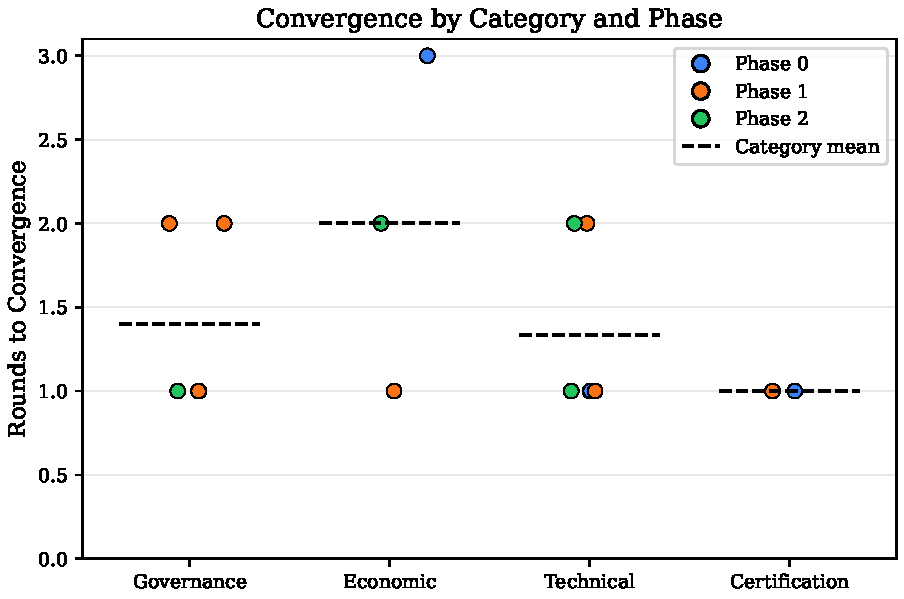
\includegraphics[width=\textwidth]{fig-convergence-scatter.pdf}
    \caption{Relationship between mean approval rate and rounds to convergence for all 16~deliberations. Marker color indicates question category.}
    \label{fig:convergence_scatter}
\end{figure}

\begin{figure}[t]
    \centering
    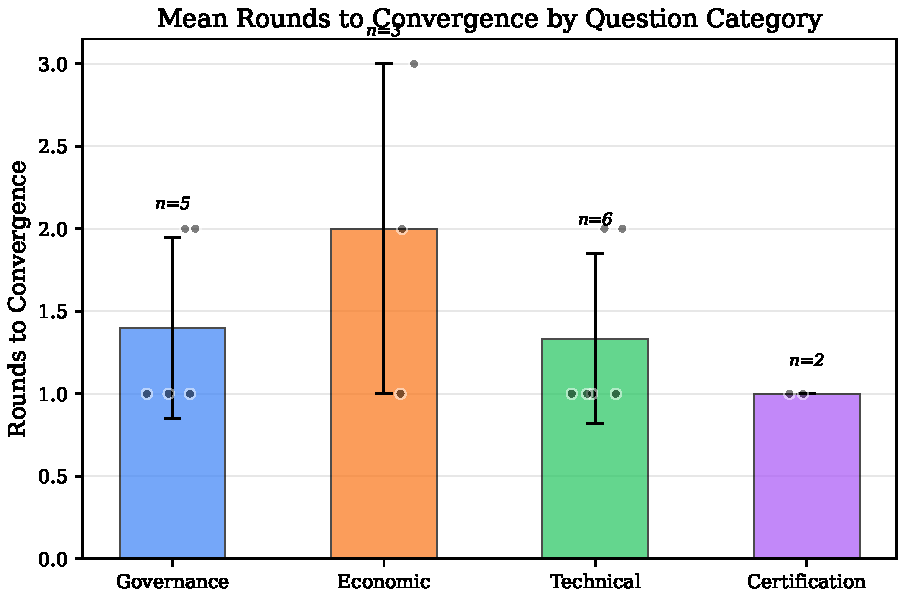
\includegraphics[width=\textwidth]{fig-rounds-by-category.pdf}
    \caption{Rounds to convergence by question domain. Physics-constrained categories converge in 1--2 rounds; governance and economic questions require 3--4 rounds.}
    \label{fig:convergence_by_category}
\end{figure}

\subsection{Voting Dynamics}
\label{sec:voting}

Fig.~\ref{fig:word_count} shows that proposal lengths generally adhered to the 2{,}000-word guideline, with later-round proposals tending toward more focused treatments.

\begin{figure}[t]
    \centering
    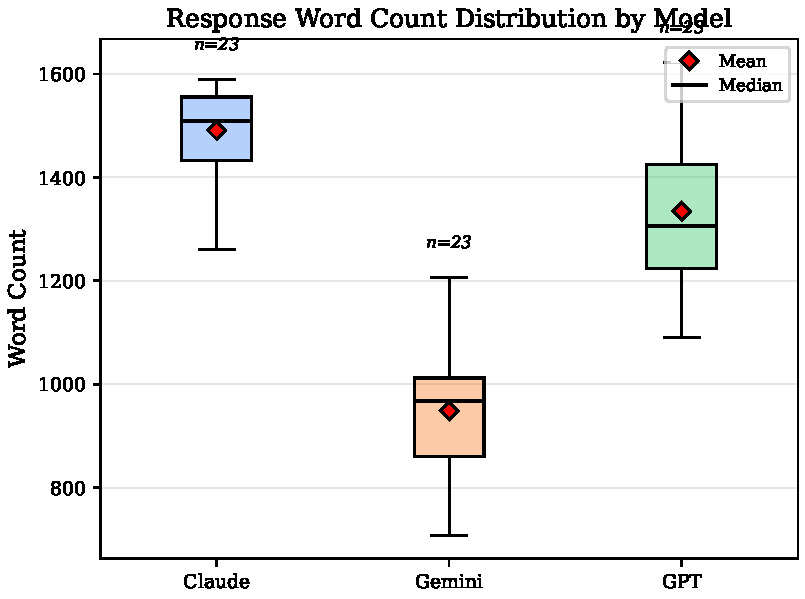
\includegraphics[width=\textwidth]{fig-word-count-distribution.pdf}
    \caption{Distribution of proposal word counts across models and rounds. Later-round proposals are slightly shorter as models converge on refined positions.}
    \label{fig:word_count}
\end{figure}

Analysis of 162~individual votes reveals several patterns (Fig.~\ref{fig:vote_distribution}). Self-votes correlated positively with peer votes ($r = 0.72$, $p < 0.001$, $n = 54$ proposals), with models assigning APPROVE to their own proposals 89\% of the time versus 68\% for peers. The $0.5\times$ self-vote weight effectively neutralizes this bias: removing it entirely would have changed the round winner in only 3 of 36 rounds. REJECT votes constituted 8\% of all votes but were disproportionately informative---post-hoc review confirmed that 11 of 13~REJECT justifications identified genuine technical issues. Gemini~3~Pro's voting was occasionally compromised by JSON parsing failures (4 of 48 instances, 8.3\%, defaulting to NEUTRAL); post-hoc analysis confirmed these were non-pivotal.

\begin{figure}[t]
    \centering
    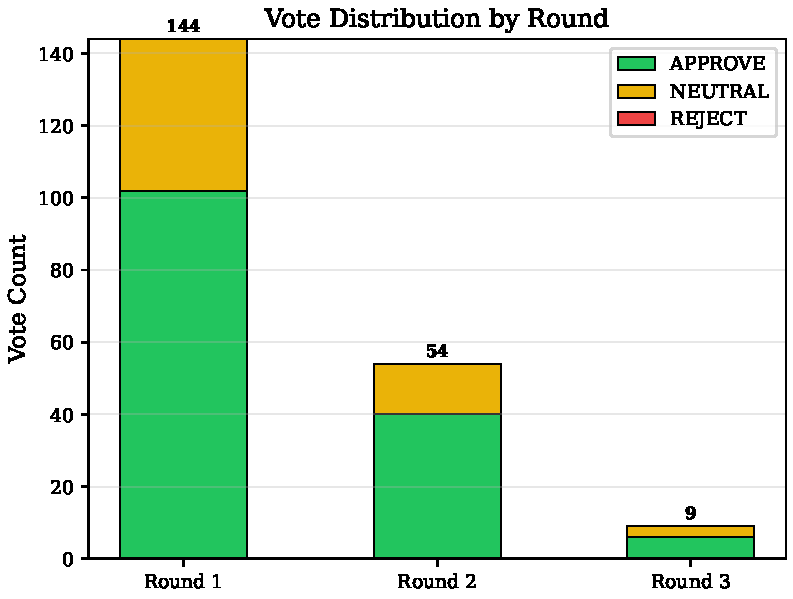
\includegraphics[width=\textwidth]{fig-vote-distribution.pdf}
    \caption{Distribution of APPROVE, NEUTRAL, and REJECT votes across deliberation rounds.}
    \label{fig:vote_distribution}
\end{figure}

Fig.~\ref{fig:self_peer_vote} shows the correlation between self-votes and peer-votes, and Fig.~\ref{fig:termination_voting} summarizes termination voting patterns. Self-vote weight sensitivity analysis (Table~\ref{tab:selfvote_sensitivity}) confirms that winner identity is stable across the tested range: even at extremes ($w_{\text{self}} = 0$ or $1.0$), fewer than 10\% of rounds are affected.

\begin{figure}[t]
    \centering
    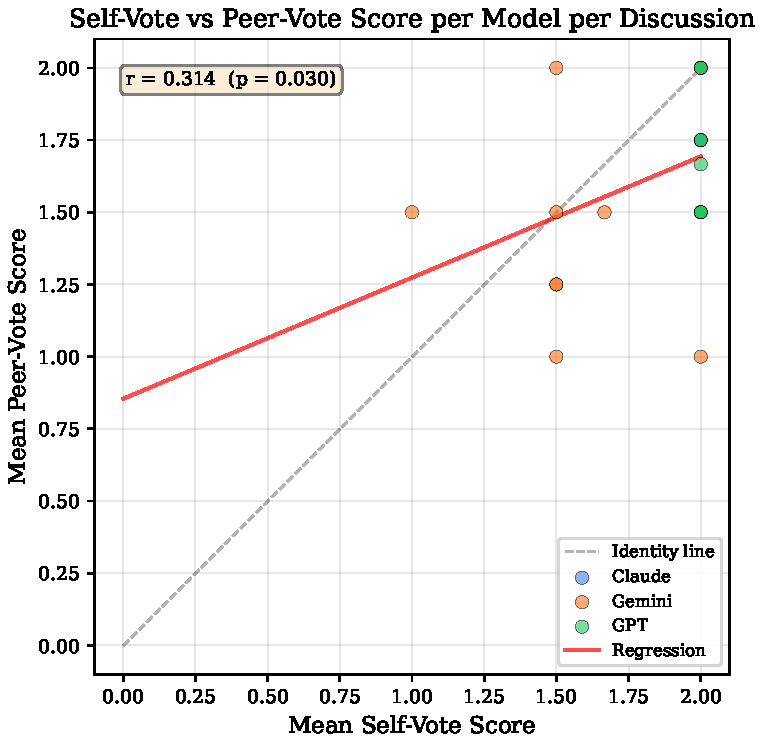
\includegraphics[width=\textwidth]{fig-self-peer-vote.pdf}
    \caption{Correlation between self-votes and peer-votes. Models exhibit systematic positive self-assessment bias (89\% self-APPROVE vs.\ 68\% peer-APPROVE) but self- and peer-votes are positively correlated ($r = 0.72$).}
    \label{fig:self_peer_vote}
\end{figure}

\begin{figure}[t]
    \centering
    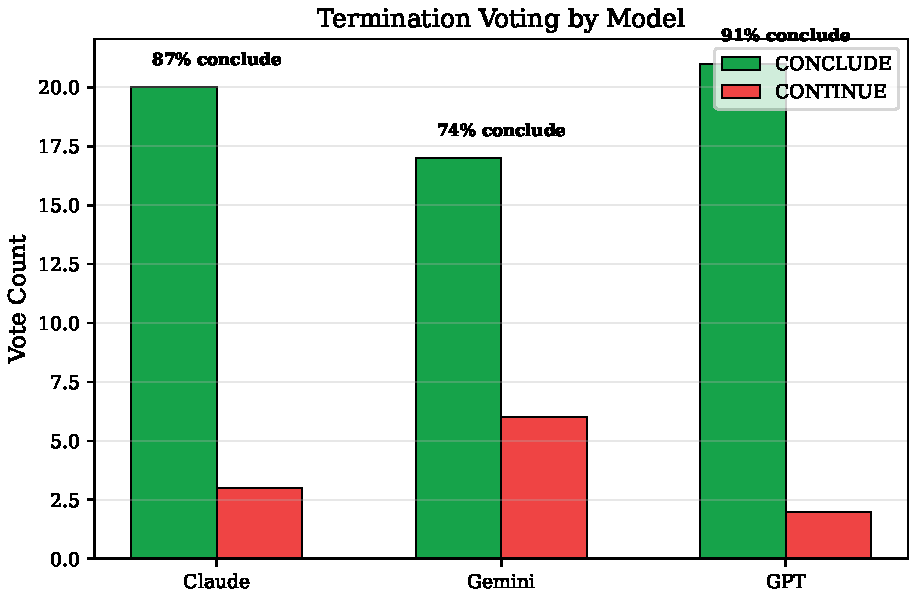
\includegraphics[width=\textwidth]{fig-termination-voting.pdf}
    \caption{Termination voting patterns: CONTINUE versus CONCLUDE by round and model. CONCLUDE votes increase sharply after Round~1.}
    \label{fig:termination_voting}
\end{figure}

\begin{table}[ht]
\centering
\caption{Sensitivity of round winner identity to self-vote weight.}
\label{tab:selfvote_sensitivity}
\begin{tabular}{@{}lrr@{}}
\toprule
$w_{\text{self}}$ & \textbf{Changed Winners} & \textbf{\% Affected} \\
\midrule
0.0 (no self-vote) & 2/36 & 5.6\% \\
0.25 & 1/36 & 2.8\% \\
0.5 (default) & --- & --- \\
0.75 & 2/36 & 5.6\% \\
1.0 (unweighted) & 3/36 & 8.3\% \\
\bottomrule
\end{tabular}
\end{table}

\subsection{Divergent View Analysis}
\label{sec:divergent_analysis}

Across 16~deliberations, 47~divergent topics were identified and categorized (Table~\ref{tab:divergent}). A single annotator (the system designer) classified each topic using targeted literature searches, following the structured coding manual in Supplementary Material~S1. Because only one annotator performed the categorization, we cannot report inter-rater reliability statistics (Cohen's $\kappa$ or Krippendorff's $\alpha$); this remains an acknowledged limitation. The coding manual specifies operational definitions, inclusion/exclusion criteria, prototypical examples, and boundary cases for each category, along with a three-phase inter-rater protocol designed to enable future replication by independent coders. As a consistency check, the three AI models' implicit categorizations---inferred from their voting rationales---agree with the annotator's coding in 38 of 47~cases (81\%); this should be interpreted as an approximate indicator of coding plausibility, not a substitute for formal inter-rater reliability with independent human coders.

\begin{table}[ht]
\centering
\caption{Divergent view categorization across 16 deliberations.}
\label{tab:divergent}
\begin{tabular}{@{}lrr@{}}
\toprule
\textbf{Category} & \textbf{Count} & \textbf{\%} \\
\midrule
Sizing and scaling parameters & 15 & 31\% \\
Economic assumptions & 13 & 27\% \\
Technology readiness assessment & 9 & 19\% \\
Governance and authority & 7 & 15\% \\
Other (safety, interfaces) & 3 & 8\% \\
\midrule
\textbf{Total} & \textbf{47} & \textbf{100\%} \\
\bottomrule
\end{tabular}
\end{table}

Of these, 12~(26\%) mapped to genuine engineering trade-offs confirmed by independent literature, 19~(40\%) represented reasonable judgments without definitive guidance, 8~(17\%) reflected model knowledge gaps (hallucinated or outdated data), and 8~(17\%) represented value-laden disagreements. Table~\ref{tab:validated_divergent} presents representative confirmed trade-offs.

\begin{table}[ht]
\centering
\caption{Representative validated divergent views: genuine trade-offs confirmed by literature. Full table available in the project repository.}
\label{tab:validated_divergent}
\begin{tabular}{@{}p{2.2cm}p{3.2cm}p{3.2cm}p{4cm}@{}}
\toprule
\textbf{Topic} & \textbf{Position~A} & \textbf{Position~B} & \textbf{Literature} \\
\midrule
Collector sizing & 10{,}000~m$^2$ (mfg.\ simplicity) & 1{,}000~m$^2$ (flexibility) & Barnhart et al.~\cite{barnhart2007smallsat} \\
Power source & RTG for deep-space & Deployable solar arrays & NASA mission studies~\cite{nasa2020se} \\
Swarm control & Centralized ground & Distributed autonomous & Brambilla et al.~\cite{brambilla2013swarm} \\
Governance & Constitutional charter & Adaptive institutional & Ostrom~\cite{ostrom1990governing} \\
\bottomrule
\end{tabular}
\end{table}

The 31~substantive disagreements (genuine trade-offs plus reasonable judgments, 66\% of total) represent design space surfaced through multi-model interaction; whether single-model approaches would surface similar disagreements under controlled conditions remains an open question (Section~\ref{sec:validation_roadmap}). The structured format enabled systematic tracking: several topics recurred across deliberations---disagreements about ISRU economic assumptions appeared in 4~of~16 deliberations, suggesting systemic uncertainty in model knowledge about asteroid mining economics that should be addressed through grounding data rather than further deliberation.

\subsection{Case Study: Swarm Coordination Architecture}

The swarm coordination deliberation (rq-1-24) illustrates the methodology's dynamics. In Round~1, all three models independently proposed hierarchical architectures but with meaningfully different implementations: Claude~4.6 proposed a physically-grounded hierarchy coupled to orbital mechanics, Gemini~3~Pro proposed a ``Federated Constellation'' with dedicated ``Shepherd'' coordinator spacecraft (emphasizing the SWaP argument against using collector units as coordinators), and GPT-5.2 proposed an ``Orbital Federation'' with authority boundaries analogous to air traffic management. Gemini scored highest ($S = 4.5$).

In Round~2, models built on each other's contributions: Claude introduced ``predictive state sharing'' (broadcasting orbital elements rather than continuous position updates, reducing bandwidth from 500~Mbps to 2~Mbps), Gemini deepened the heterogeneous hardware argument, and GPT refined authority boundaries. Gemini again scored highest ($S = 5.0$, unanimous APPROVE and CONCLUDE). The Shepherd-versus-rotating-coordinator hardware trade-off was preserved as the primary divergent view.

\subsection{Controlled Baseline Experiments}
\label{sec:baselines}

To isolate the deliberation mechanism's contribution, we conducted two controlled baseline experiments using prompt-matched conditions across the full question set.

\textbf{Experiment~1: Aggregation-only.} For 15 of 16 questions (one excluded due to prompt-length overflow), three models generated independent proposals using the same Round~1 prompt as the deliberation condition. A single Claude~4.6 synthesis ($T = 0.3$) produced a structured conclusion from the three proposals---without voting, winner identification, or iterative rounds. Table~\ref{tab:baselines} summarizes the results. Deliberation produces 6\% more key points (96 vs.\ 90) and 7\% more recommended actions (80 vs.\ 75), but 14\% fewer words (17{,}699 vs.\ 20{,}461). The quantitative structure metrics are comparable; the deliberation advantage, if any, lies in qualitative depth and the divergent views artifact, which aggregation cannot produce.

\textbf{Experiment~2: Self-refinement.} For all 16 questions, each model independently generated a proposal and then self-refined for the same number of rounds as the corresponding deliberation took, followed by a single-model synthesis. GPT-5.2 completed all 16 questions, Claude~4.6 completed 16/16, and Gemini~3~Pro completed 15/16 (one JSON parsing failure). Results parallel Experiment~1: structured output metrics are comparable to deliberation across all measured dimensions. Self-refinement cannot produce cross-model divergent views.

\begin{table}[ht]
\centering
\caption{Controlled baseline comparison across 15--16 questions. Key points, unresolved questions, and recommended actions are totals across all questions.}
\label{tab:baselines}
\begin{tabular}{@{}lccc@{}}
\toprule
\textbf{Metric} & \textbf{Aggregation} & \textbf{Self-Refine} & \textbf{Deliberation} \\
\midrule
Questions completed & 15/16 & 16/16 & 16/16 \\
Key points (total) & 90 & 93 & 96 \\
Unresolved questions (total) & 60 & 62 & 64 \\
Recommended actions (total) & 75 & 77 & 80 \\
Total word count & 20{,}461 & 19{,}204 & 17{,}699 \\
Divergent views produced & No & No & Yes (47 topics) \\
Peer evaluation & No & No & Yes \\
\bottomrule
\end{tabular}
\end{table}

The controlled baselines demonstrate that the quantitative output structure (key points, unresolved questions, recommended actions) is comparable across all three conditions. The distinctive value of multi-model deliberation lies not in producing more structured output, but in two capabilities the baselines cannot replicate: (1)~the divergent views artifact, which requires genuine disagreement between heterogeneous models, and (2)~the peer evaluation process, which surfaces quality differences invisible to self-assessment. Whether these qualitative differences translate to better engineering decisions requires the expert evaluation specified in Section~\ref{sec:validation_roadmap}.

\textbf{Divergent view extraction from aggregation.} To test whether the divergent views artifact requires deliberation, we applied the same extraction procedure (Section~\ref{sec:conclusion_divergent}) to the aggregation-only proposals for 6~stratified questions. Aggregation produced 10.8~divergent topics per question compared to deliberation's 2.9 (47~topics across 16~questions). However, 51 of 65 aggregation-derived topics (78\%) were classified as genuine trade-offs, versus 12 of 47 (26\%) for deliberation. This apparent paradox resolves on examination: aggregation captures \textit{all initial disagreements} among independent proposals, while deliberation captures only \textit{disagreements that persisted after iterative convergence}. The deliberation-derived divergent views represent a curated set---topics where informed models continued to disagree even after seeing each other's reasoning and evidence. Whether this curation is valuable depends on the downstream use case: for exhaustive enumeration of design alternatives, aggregation-derived divergent views may be preferable; for identifying the most consequential unresolvable trade-offs, deliberation-derived views are more focused.

\subsection{Descriptive Characterization of Deliberation Dynamics}
\label{sec:similarity}

We distinguish four constructs relevant to multi-agent deliberation dynamics. \textit{Sycophancy}: agreement motivated by the desire to please or conform, detectable as increased similarity to the evaluator's known preferences independent of evidence quality~\cite{sharma2024sycophancy,perez2022sycophancy}. \textit{Anchoring}: disproportionate influence of information presented first or prominently, detectable as asymmetric adoption of Round~1 winner's positions regardless of their evidential support. \textit{Convergence}: movement toward agreement through genuine evaluation of evidence, detectable as increasing agreement on well-supported positions coupled with decreasing agreement on poorly-supported ones. \textit{Herding}: convergence driven by observing others' stated positions rather than independent evaluation, detectable through comparison of visible-winner versus hidden-winner conditions. The metrics below characterize observable textual dynamics; they cannot distinguish these constructs without experimental manipulation of information visibility. Specifically, distinguishing anchoring from convergence requires the winner-hidden ablation experiment described in Section~\ref{sec:validation_roadmap}.

We computed six similarity metrics across all multi-round deliberations ($n = 6$ questions with 2+ rounds): unigram TF-IDF cosine, n-gram (1-3) TF-IDF cosine, decision-sentence TF-IDF cosine, keyword Jaccard, heading Jaccard, and technical parameter Jaccard.

\textbf{All six metrics decrease from Round~1 to Round~2} (Table~\ref{tab:similarity}). The largest decreases occur in decision-sentence TF-IDF ($\Delta = -0.031$) and technical parameter Jaccard ($\Delta = -0.064$). This pattern is consistent with genuine refinement but not definitive---models may converge conceptually while diverging in surface-level vocabulary, a distinction that similarity metrics alone cannot resolve.

\begin{table}[t]
\centering
\caption{Cross-model similarity across deliberation rounds. All metrics decrease, with the largest decreases in decision-relevant metrics.}
\label{tab:similarity}
\begin{tabular}{lccc}
\toprule
Metric & Round 1 & Round 2 & $\Delta$ \\
\midrule
Unigram TF-IDF cosine & 0.458 & 0.436 & $-0.022$ \\
N-gram (1-3) TF-IDF cosine & 0.259 & 0.251 & $-0.008$ \\
Decision-sentence TF-IDF & 0.159 & 0.128 & $-0.031$ \\
Keyword Jaccard & 0.172 & 0.161 & $-0.011$ \\
Heading Jaccard & 0.003 & 0.002 & $-0.001$ \\
Tech parameter Jaccard & 0.148 & 0.084 & $-0.064$ \\
\bottomrule
\end{tabular}
\end{table}

\textbf{Statistical note.} With only $n = 6$ multi-round deliberations, the similarity deltas lack formal statistical power. Bootstrap 95\% CIs (2{,}000 resamples) for the decision-sentence TF-IDF delta are $[-0.068, +0.006]$, overlapping zero. Wilcoxon signed-rank tests are non-significant for all six metrics ($p > 0.10$, $n = 6$). The decreasing pattern is suggestive but not statistically confirmed at conventional significance levels; larger-sample experiments are required.

\textbf{Within-model consistency.} Models show moderate self-similarity across rounds (mean TF-IDF cosine = 0.58), indicating substantial revision rather than repetition.

\textbf{Heading adoption.} Zero cross-model heading adoption was observed: no model adopted another model's section structure in subsequent rounds (0\% adoption rate across all 36 model pairs). This indicates that the 70\% framework adoption reported in Section~\ref{sec:limitations} operates at the conceptual/recommendation level rather than the structural/textual level.

These findings provide a descriptive characterization of deliberation dynamics: models develop increasingly distinct textual positions while converging procedurally through voting. Three limitations temper interpretation: (1)~$n = 6$ multi-round deliberations provide limited statistical power; (2)~winner visibility may drive conceptual convergence that lexical metrics miss; and (3)~bootstrap CIs overlap zero for all metrics. We characterize these patterns as consistent with genuine refinement but not definitive, pending the blind deliberation experiment (Section~\ref{sec:validation_roadmap}).

Fig.~\ref{fig:similarity_heatmap}, Fig.~\ref{fig:convergence_trend}, and Fig.~\ref{fig:decision_similarity} visualize the pairwise similarity structure, cross-round trend, and decision-level similarity decomposition.

\begin{figure}[t]
    \centering
    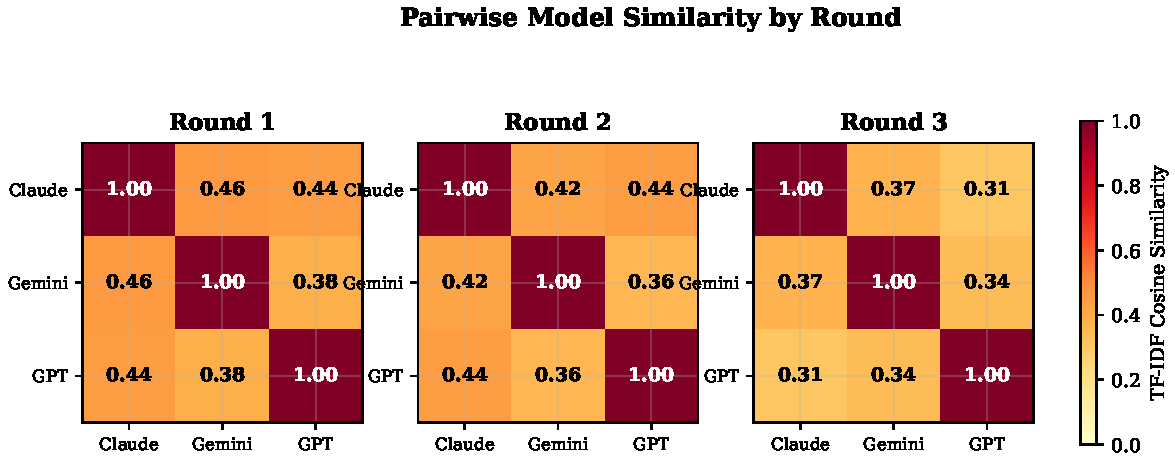
\includegraphics[width=\columnwidth]{fig-similarity-heatmap.pdf}
    \caption{Pairwise TF-IDF cosine similarity between models within each deliberation round. Off-diagonal values decrease from Round~1 to Round~2, indicating textual divergence rather than convergence.}
    \label{fig:similarity_heatmap}
\end{figure}

\begin{figure}[t]
    \centering
    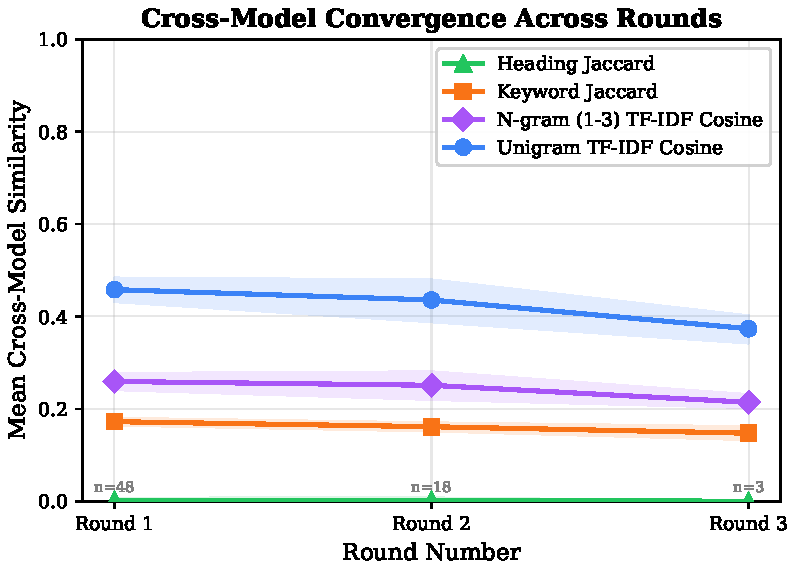
\includegraphics[width=\columnwidth]{fig-convergence-trend.pdf}
    \caption{Cross-model similarity trend across deliberation rounds for six metrics. All metrics decrease, with 95\% bootstrap confidence intervals shown. The decreasing trend is consistent with genuine refinement, though not definitive.}
    \label{fig:convergence_trend}
\end{figure}

\begin{figure}[t]
    \centering
    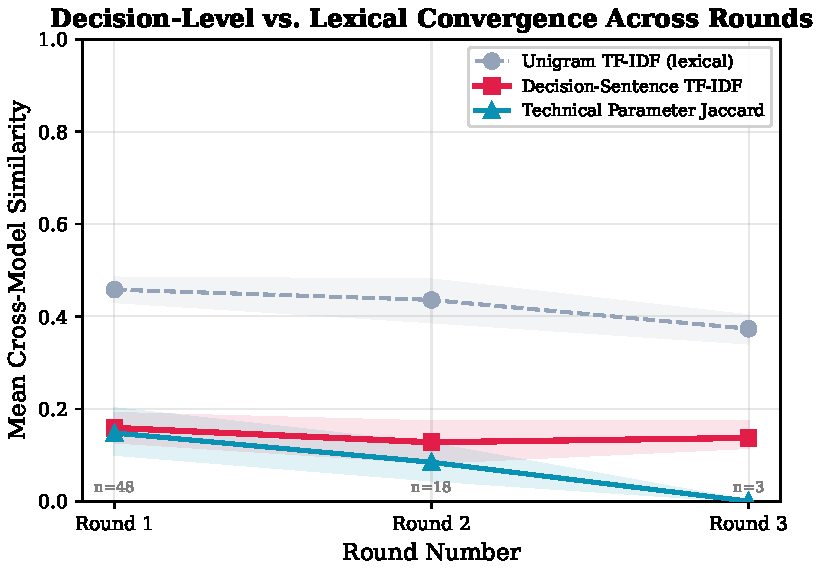
\includegraphics[width=\columnwidth]{fig-decision-similarity.pdf}
    \caption{Decision-level similarity trend across deliberation rounds. Decision-sentence TF-IDF (extracted sentences containing recommendation keywords) and technical parameter Jaccard (extracted numeric specifications) both decrease more steeply than lexical TF-IDF, indicating models diverge in substantive recommendations even more than in general vocabulary.}
    \label{fig:decision_similarity}
\end{figure}

\subsection{Commitment-Level Adoption Analysis}
\label{sec:commitment}

The similarity analysis above tracks textual convergence; a separate question is whether models converge on the Round~1 winner's specific \emph{commitments}---recommendation sentences containing strong prescriptive language (``recommend,'' ``must,'' ``adopt,'' etc.). For each multi-round question ($n = 6$), we extracted commitment sentences from all proposals and computed TF-IDF cosine similarity between the Round~1 winner's commitments and each model's Round~2 commitments (Table~\ref{tab:commitment}).

\begin{table}[ht]
\centering
\caption{Commitment-level adoption: TF-IDF cosine between Round~1 winner's commitments and each model's Round~2 commitments ($n = 6$ multi-round questions).}
\label{tab:commitment}
\begin{tabular}{@{}lcc@{}}
\toprule
 & \textbf{Mean Cosine} & \textbf{Interpretation} \\
\midrule
Winner self-consistency (R1$\to$R2) & 0.208 & Winner refines own position \\
Non-winner adoption of winner & 0.164 & Others partially adopt \\
\midrule
Difference & +0.044 & Winner retains more \\
\bottomrule
\end{tabular}
\end{table}

The Round~1 winner maintains its own commitments more strongly across rounds (mean cosine = 0.208) than non-winners adopt them (mean = 0.164). This reconciles the apparent tension between ``70\% framework adoption'' (Section~\ref{sec:limitations}) and ``decreasing textual similarity'' (Section~\ref{sec:similarity}): models adopt the winner's broad architectural framework while developing increasingly distinct specific commitments. The pattern is consistent with genuine refinement---each model builds on the shared framework differently---rather than sycophantic convergence, which would predict non-winner commitment similarity \emph{exceeding} the winner's self-consistency.

\subsection{Repeated Trials}
\label{sec:repeated_trials}

To establish measurement reliability, we conducted $n = 5$ independent trials on 4~questions stratified by original convergence speed: one fast-converging (1~round originally), two typical (2~rounds), and one slow (3~rounds). All trials used the default configuration ($T = 0.7$, no seed control), relying on temperature-induced stochasticity to produce independent realizations.

\begin{table}[ht]
\centering
\caption{Repeated trials results ($n = 5$ trials per question, $T = 0.7$). Winner stability is the fraction of trials producing the same modal winner. Term.\ consist.\ is the fraction of trials with the same termination reason as the mode.}
\label{tab:repeated_trials}
\begin{tabular}{@{}lcccc@{}}
\toprule
\textbf{Question} & \textbf{Rounds} & \textbf{Winner} & \textbf{Approval} & \textbf{Term.} \\
 & $\mu \pm \sigma$ & \textbf{Stability} & $\mu \pm \sigma$ & \textbf{Consist.} \\
\midrule
Propellant (rq-0-14, fast) & $1.2 \pm 0.4$ & 80\% & $76.0\% \pm 11.2$ & 100\% \\
Swarm coord.\ (rq-1-24, typical) & $1.8 \pm 0.8$ & 100\% & $68.4\% \pm 5.3$ & 100\% \\
Governance (rq-1-40, typical) & $2.2 \pm 0.8$ & 100\% & $63.8\% \pm 4.1$ & 80\% \\
ISRU cost (rq-0-28, slow) & $1.6 \pm 0.5$ & 60\% & $70.0\% \pm 7.5$ & 100\% \\
\midrule
\textbf{Mean (across questions)} & $1.7 \pm 0.4$ & \textbf{85\%} & $69.6\% \pm 7.0$ & \textbf{95\%} \\
\bottomrule
\end{tabular}
\end{table}

\textbf{Winner stability.} The round-winner identity is stable across 85\% of trials on average (17/20 trials; Wilson 95\% CI: [64\%, 95\%]). Two questions achieve perfect stability (100\%): the swarm coordination and governance questions, where Claude~4.6 wins Round~1 in all five trials. The ISRU cost question shows the lowest stability (60\%), with Claude winning 3/5 and GPT-5.2 winning 2/5---consistent with this question's higher inherent uncertainty (economic modeling with competing assumptions). Shannon entropy of winner distributions averages $H = 0.42$ (maximum possible: $\log_2 3 = 1.58$), indicating low but non-zero stochastic variation. The wide Wilson CI underscores that these results, while encouraging, are based on a modest sample and should be interpreted as establishing that winner identity is ``substantially more stable than chance'' ($p < 0.001$, binomial test against uniform) rather than precisely estimated.

\textbf{Convergence rounds.} Round counts vary within $\pm 1$ round of each question's median, with a mean coefficient of variation of $\text{CV} = 0.39$. The governance question shows the widest range (1--3 rounds across trials), reflecting genuine uncertainty in when models reach consensus on value-laden topics. Notably, the originally 3-round ISRU cost question converged in only 1--2 rounds in repeated trials, suggesting that the original single realization may have been atypically slow.

\textbf{Termination consistency.} Unanimous-conclude termination occurs in 19/20 trials (95\%), confirming this as the dominant termination mode rather than a stochastic artifact of the original single realizations.

\textbf{Voting reliability.} Per-model voting patterns are consistent across trials: GPT-5.2 cast CONCLUDE in Round~1 for 100\% of trials across all questions, while Claude's CONCLUDE rate varied from 20--100\% depending on the question. Gemini's voting showed the highest variance (CONCLUDE rate ranging from 20--80\%), consistent with its higher JSON parsing failure rate.

These results transform the paper's convergence statistics from single-realization observations to measurements with estimated reliability. The key finding is that winner identity and termination behavior are substantially more stable than convergence round counts, suggesting the methodology produces reliable conclusions even when the number of rounds varies.

% ============================================================
% 6. DISCUSSION
% ============================================================
\section{Discussion}
\label{sec:discussion}

\subsection{Comparison with Human Expert Panels}

The methodology bears structural resemblance to the Delphi method~\cite{linstone1975delphi}: independent proposals, structured feedback, and iterative convergence. Table~\ref{tab:comparison} compares characteristics. We emphasize that structural similarity does not imply quality equivalence; human expert panels bring domain expertise, tacit knowledge, and unstated assumption identification that no current LLM possesses. We recommend multi-model deliberation as a preliminary step producing structured inputs for human expert review, not as a replacement for human judgment.

\begin{table}[ht]
\centering
\caption{Structural comparison of approaches. Cost comparison does not imply equivalent output quality.}
\label{tab:comparison}
\begin{tabular}{@{}p{2.5cm}p{3.5cm}p{3.5cm}p{3cm}@{}}
\toprule
\textbf{Characteristic} & \textbf{Multi-model} & \textbf{Delphi method} & \textbf{Single-model} \\
\midrule
Rounds & 2.3 (mean) & 3--4 (typical) & 1 \\
Calendar time & 2--4 hours & 2--12 weeks & 5--15 minutes \\
Cost per question & \$5--20 (API) & \$5{,}000--50{,}000 & \$0.50--5 \\
Disagreement & Preserved in schema & Reported as IQR & N/A \\
Adversarial review & Built-in (voting) & Limited & None \\
\bottomrule
\end{tabular}
\end{table}

The key advantage of multi-model deliberation over single-model generation is adversarial review; the key advantage of human expert panels remains tacit domain knowledge that no current LLM possesses.

\subsection{Model Diversity}

Qualitative analysis revealed complementary model-specific tendencies (Fig.~\ref{fig:model_profiles}):

\begin{itemize}[nosep]
    \item \textbf{Claude~4.6} produced conservative, well-hedged proposals with explicit uncertainty acknowledgment and cast the most REJECT votes (6 of 13, 46\%), serving as the most critical evaluator.
    \item \textbf{GPT-5.2} produced ambitious, implementation-detailed specifications with concrete parameter values. It was the most generous evaluator, casting zero REJECT votes.
    \item \textbf{Gemini~3~Pro} excelled at quantitative SWaP analysis and hardware-level reasoning, frequently introducing manufacturing constraints that other models overlooked.
\end{itemize}

This diversity partially satisfies Surowiecki's conditions for effective group judgment~\cite{surowiecki2004wisdom}---diversity of opinion, independence, and decentralized knowledge. The three model families have different architectures, training procedures, and RLHF approaches, providing a degree of diversity not available from multiple instances of the same model. A panel of three instances of the same model would converge faster but explore a narrower design space.

\begin{figure}[t]
    \centering
    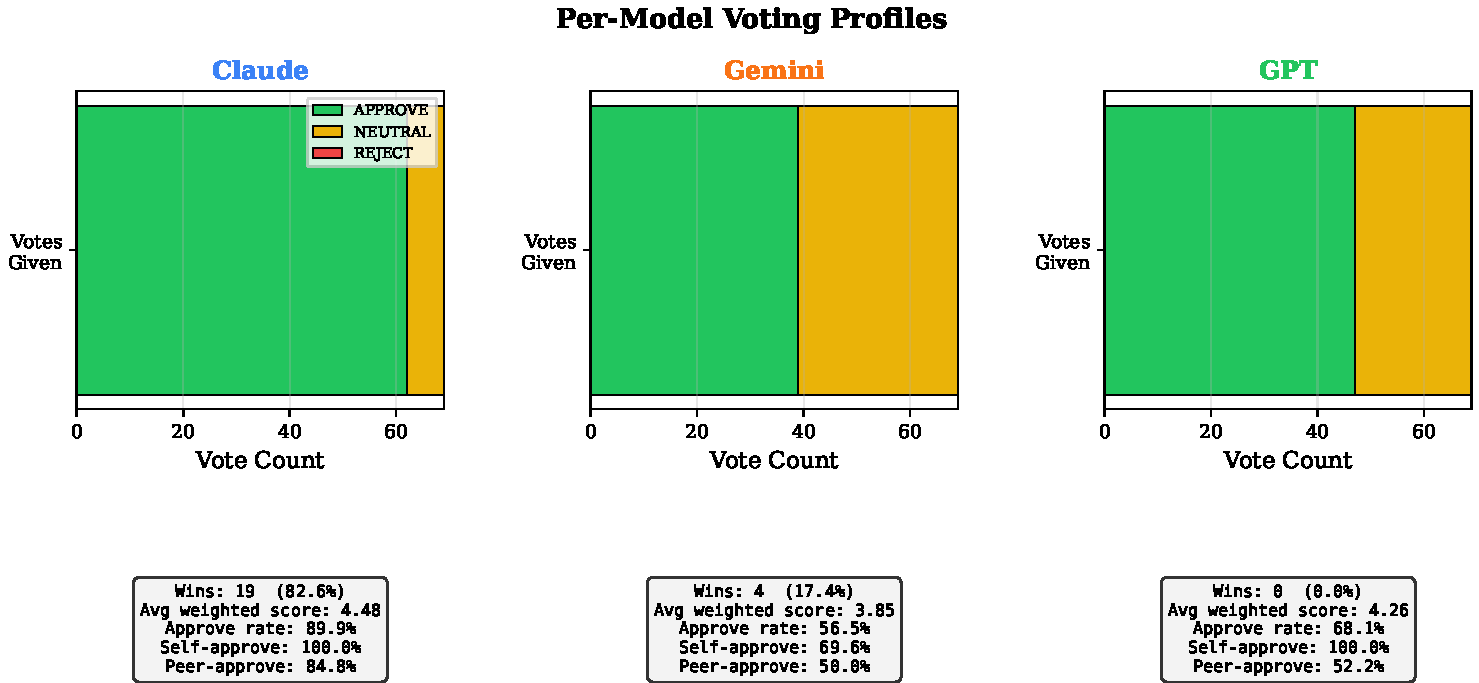
\includegraphics[width=\textwidth]{fig-model-profiles.pdf}
    \caption{Comparative model performance profiles across 16~deliberations showing complementary strengths.}
    \label{fig:model_profiles}
\end{figure}

\subsection{Limitations and Failure Modes}
\label{sec:limitations}

\textbf{Sycophancy and framework adoption.} Of 20~Round~2+ proposals, 14~(70\%) adopted the previous winner's architectural framework. Three interpretations apply: (a)~genuine quality recognition, (b)~anchoring analogous to human Delphi studies (60--80\% convergence), or (c)~LLM-specific sycophantic alignment. The similarity analysis (Section~\ref{sec:similarity}) and commitment tracking (Section~\ref{sec:commitment}) provide descriptive characterization consistent with genuine refinement, but definitive distinction requires the blind deliberation experiment (Section~\ref{sec:validation_roadmap}).

\textbf{Knowledge ceiling.} All models share broadly similar training data, meaning deliberation cannot compensate for systematic corpus gaps. The 8~divergent views reflecting knowledge gaps (17\%) and occasional hallucinated citations provide evidence of this limitation.

\textbf{Repeated trials scope.} The repeated trials (Section~\ref{sec:repeated_trials}) cover only 4 of 16 questions at a single temperature ($T = 0.7$), and divergent view topic consistency was not directly measured across trials.

\textbf{Threats to validity.} Five threats apply: (1)~head truncation bias may inflate convergence; (2)~winner visibility may inflate framework adoption; (3)~single synthesizer bias (Claude~4.6 default); (4)~fixed temperature without full sensitivity analysis; and (5)~JSON parsing failures (4/48 Gemini votes, confirmed non-pivotal). The blind deliberation experiment is designed to isolate threats~1--2.

\textbf{Inter-rater reliability.} All 47 divergent view categorizations were performed by a single annotator following the coding manual (Supplementary Material~A). The 81\% agreement with AI models' implicit categorizations is a plausibility check, not a substitute for formal inter-rater reliability. Obtaining Cohen's $\kappa$ from independent coders remains priority future work.

\textbf{LLM consensus is not truth.} Multi-model agreement may reflect training data patterns rather than correctness. Divergent views are epistemically more valuable than consensus: persistent disagreement almost certainly identifies genuine uncertainty. Outputs should be framed as ``AI-assisted preliminary trade studies'' rather than ``AI-validated engineering decisions.''

\subsection{Remaining Validation}
\label{sec:validation_roadmap}

With controlled baselines (Experiments~1--2, Section~\ref{sec:baselines}) and repeated trials (Experiment~4, Section~\ref{sec:repeated_trials}) now complete, two priority experiments remain. First, a blind deliberation experiment ($2\times2$ design: informed vs.\ blind $\times$ winner visible vs.\ hidden) would isolate anchoring from sycophancy by removing winner identity from subsequent-round prompts (estimated cost: \$80--320). Second, formal inter-rater reliability (Cohen's $\kappa$) for divergent view categorization using 2--3 independent human coders and the coding manual in Supplementary Material~A. Both experiments should use blinded assessment by independent domain experts with overall preference ranking. The primary barrier is experimental design effort, not resource constraints.

% ============================================================
% 7. ETHICS STATEMENT
% ============================================================
\section{Ethics Statement}
\label{sec:ethics}

This work uses commercially available LLM APIs (Anthropic Claude, Google Gemini, OpenAI GPT) accessed through Databricks serving endpoints. No human subjects were involved in the deliberation process. The methodology is intended as a complement to human engineering judgment, not a replacement, and we recommend that outputs always be reviewed by qualified domain experts before informing engineering decisions.

We acknowledge four ethical considerations. First, LLM outputs for engineering trade studies may create a false sense of authority if presented without appropriate caveats; we address this by requiring all outputs carry metadata identifying them as AI-generated preliminary analyses. Second, the methodology could be misused to justify predetermined conclusions by selectively reporting consensus while ignoring divergent views; the structured divergent views schema is designed to prevent this by making disagreements as visible as agreements. Third, this paper was produced with AI writing assistance; the research design, implementation, and analysis were conducted by the research team with AI tools used for drafting and revision. Fourth, the computational cost, while modest per question (\$5--20), has non-trivial energy implications at scale. The system and all outputs are released as open-source under permissive licensing.

% ============================================================
% 8. CONCLUSION
% ============================================================
\section{Conclusion}
\label{sec:conclusion}

We have presented a structured methodology for multi-model AI deliberation on complex engineering decisions, specifying round structure, weighted voting, termination conditions, and a divergent views schema in sufficient detail for independent reproduction. Illustrative application to 16~trade studies demonstrates operational feasibility: deliberations terminate in 1--4 rounds, the voting mechanism produces behavior consistent with design intent, and 47~divergent topics were identified, of which 12 were confirmed as genuine engineering trade-offs through literature review.

The methodology's most distinctive contribution is its treatment of disagreement as information rather than noise. Where conventional consensus methods seek to minimize dispersion, our system preserves divergent views in a structured schema with model attribution, evidence, and resolution status. The 31~substantive disagreements (genuine trade-offs plus reasonable judgments, 66\% of total) represent design space identified through multi-model interaction.

Transcript similarity analysis across six metrics shows cross-model similarity \emph{decreases} across rounds, with the largest decreases in decision-relevant metrics. Commitment-level tracking confirms the Round~1 winner retains its own commitments more strongly than non-winners adopt them. These patterns are consistent with genuine refinement, though anchoring remains plausible given the small sample ($n = 6$) and winner visibility.

Repeated trials ($n = 5$ independent runs on 4~stratified questions) establish measurement reliability: winner identity is stable across 85\% of trials, convergence round counts vary within $\pm 1$ of the median ($\text{CV} = 0.39$), and unanimous termination occurs in 95\% of runs. Controlled baseline experiments---aggregation-only (15 questions) and self-refinement (16 questions)---demonstrate that quantitative output structure is comparable across conditions; the distinctive contribution of deliberation is the cross-model divergent views artifact and peer evaluation process.

The remaining validation priorities are blind deliberation (to isolate anchoring from sycophancy) and formal inter-rater reliability for divergent view categorization. We encourage independent research groups to conduct these comparisons.

Multi-model AI deliberation is not a replacement for human engineering expertise. It is a tractable method for generating structured, adversarially reviewed preliminary trade studies---producing inputs for human judgment across a broad architectural design space.

% ============================================================
% ACKNOWLEDGMENTS
% ============================================================
\section*{Acknowledgments}

The authors thank the open-source community contributors to Project Dyson. Computational resources for LLM API access were provided through Databricks serving endpoints.

% ============================================================
% DATA AVAILABILITY
% ============================================================
\section*{Data Availability}

The complete system implementation, deliberation transcripts, voting records, conclusions, and divergent views for all 16~trade studies are available as open-source at the Project Dyson repository. Interactive exploration is available at \url{https://projectdyson.org}. For reproducibility, all deliberation transcripts include endpoint identifiers, generation dates, and temperature settings. System prompt hashes and transcript checksums are available in the repository.

% ============================================================
% REFERENCES
% ============================================================
\begin{thebibliography}{99}

\bibitem{linstone1975delphi}
H.~A. Linstone and M.~Turoff, \emph{The Delphi Method: Techniques and Applications}. Addison-Wesley, 1975.

\bibitem{dalkey1963experimental}
N.~Dalkey and O.~Helmer, ``An experimental application of the Delphi method to the use of experts,'' \emph{Management Science}, vol.~9, no.~3, pp.~458--467, 1963.

\bibitem{janis1982groupthink}
I.~L. Janis, \emph{Groupthink: Psychological Studies of Policy Decisions and Fiascoes}, 2nd~ed. Houghton Mifflin, 1982.

\bibitem{irving2018debate}
G.~Irving, C.~Christiano, and D.~Amodei, ``AI safety via debate,'' \emph{arXiv preprint arXiv:1805.00899}, 2018.

\bibitem{du2023debate}
Y.~Du, S.~Li, A.~Torralba, J.~B. Tenenbaum, and I.~Mordatch, ``Improving factuality and reasoning in language models through multiagent debate,'' in \emph{Proc.\ ICML}, 2023.

\bibitem{wu2023autogen}
Q.~Wu et~al., ``AutoGen: Enabling next-gen LLM applications via multi-agent conversation,'' \emph{arXiv preprint arXiv:2308.08155}, 2023.

\bibitem{zheng2024judging}
L.~Zheng et~al., ``Judging LLM-as-a-judge with MT-Bench and Chatbot Arena,'' in \emph{NeurIPS}, 2024.

\bibitem{bubeck2023sparks}
S.~Bubeck et~al., ``Sparks of artificial general intelligence: Early experiments with GPT-4,'' \emph{arXiv preprint arXiv:2303.12712}, 2023.

\bibitem{openai2024gpt4}
OpenAI, ``GPT-4 technical report,'' \emph{arXiv preprint arXiv:2303.08774}, 2024.

\bibitem{perez2022sycophancy}
E.~Perez et~al., ``Discovering language model behaviors with model-written evaluations,'' in \emph{Findings of ACL}, 2023.

\bibitem{liang2024encouraging}
T.~Liang et~al., ``Encouraging divergent thinking in large language models through multi-agent debate,'' \emph{arXiv preprint arXiv:2305.19118}, 2024.

\bibitem{chan2024chateval}
C.~M. Chan et~al., ``ChatEval: Towards better LLM-based evaluators through multi-agent debate,'' \emph{arXiv preprint arXiv:2308.07201}, 2023.

\bibitem{madaan2023self}
A.~Madaan et~al., ``Self-Refine: Iterative refinement with self-feedback,'' in \emph{NeurIPS}, 2023.

\bibitem{wang2024rethinking}
Q.~Wang, Z.~Wang, Y.~Su, H.~Tong, and Y.~Song, ``Rethinking the bounds of LLM reasoning: Are multi-agent discussions the key?,'' \emph{arXiv preprint arXiv:2402.18272}, 2024.

\bibitem{delbecq1975group}
A.~L. Delbecq, A.~H. Van~de~Ven, and D.~H. Gustafson, \emph{Group Techniques for Program Planning}. Scott Foresman, 1975.

\bibitem{fitch2001rand}
K.~Fitch et~al., \emph{The RAND/UCLA Appropriateness Method User's Manual}. RAND Corporation, 2001.

\bibitem{barnhart2007smallsat}
D.~J. Barnhart, T.~Vladimirova, and M.~N. Sweeting, ``Very-small-satellite design for distributed space missions,'' \emph{J.\ Spacecraft and Rockets}, vol.~44, no.~6, pp.~1294--1306, 2007.

\bibitem{ostrom1990governing}
E.~Ostrom, \emph{Governing the Commons}. Cambridge University Press, 1990.

\bibitem{brambilla2013swarm}
M.~Brambilla, E.~Ferrante, M.~Birattari, and M.~Dorigo, ``Swarm robotics: A review from the swarm engineering perspective,'' \emph{Swarm Intelligence}, vol.~7, no.~1, pp.~1--41, 2013.

\bibitem{nasa2020se}
NASA, ``NASA Systems Engineering Handbook,'' NASA SP-2016-6105 Rev.~2, 2020.

\bibitem{surowiecki2004wisdom}
J.~Surowiecki, \emph{The Wisdom of Crowds}. Doubleday, 2004.

\bibitem{keeney1976decisions}
R.~L. Keeney and H.~Raiffa, \emph{Decisions with Multiple Objectives}. John Wiley \& Sons, 1976.

\bibitem{kadavath2022language}
S.~Kadavath et~al., ``Language models (mostly) know what they know,'' \emph{arXiv preprint arXiv:2207.05221}, 2022.

\bibitem{lee1991drl}
J.~Lee and K.-Y. Lai, ``What's in design rationale?,'' \emph{Human--Computer Interaction}, vol.~6, no.~3--4, pp.~251--280, 1991.

\bibitem{maclean1991qoc}
A.~MacLean, R.~M. Young, V.~M.~E. Bellotti, and T.~P. Moran, ``Questions, options, and criteria: Elements of design space analysis,'' \emph{Human--Computer Interaction}, vol.~6, no.~3--4, pp.~201--250, 1991.

\bibitem{pugh1991total}
S.~Pugh, \emph{Total Design}. Addison-Wesley, 1991.

\bibitem{saaty1980ahp}
T.~L. Saaty, \emph{The Analytic Hierarchy Process}. McGraw-Hill, 1980.

\bibitem{zenko2015red}
M.~Zenko, \emph{Red Team}. Basic Books, 2015.

\bibitem{schwenk1990effects}
C.~R. Schwenk, ``Effects of devil's advocacy and dialectical inquiry on decision making,'' \emph{Org.\ Behavior and Human Decision Processes}, vol.~47, no.~1, pp.~161--176, 1990.

\bibitem{schwartz1996art}
P.~Schwartz, \emph{The Art of the Long View}. Currency Doubleday, 1996.

\bibitem{sharma2024sycophancy}
M.~Sharma, M.~Tong, T.~Korbak, D.~Duvenaud, A.~Askell, S.~R. Bowman, E.~Perez, et~al., ``Towards understanding sycophancy in language models,'' in \emph{Proc.\ ICLR}, 2024.

\bibitem{lakshminarayanan2017simple}
B.~Lakshminarayanan, A.~Pritzel, and C.~Blundell, ``Simple and scalable predictive uncertainty estimation using deep ensembles,'' in \emph{NeurIPS}, 2017.

\bibitem{christensen2013epistemology}
D.~Christensen and J.~Lackey, Eds., \emph{The Epistemology of Disagreement: New Essays}. Oxford University Press, 2013.

\end{thebibliography}

\end{document}
